\chapter{Complex Attosecond Transient-absorption Spectroscopy}
\label{chap:CATS}

\section{Introduction}
\label{sec:intro_cats}

As seen in Chapter \ref{chap:ATS}, a rich amount of information can be extracted from ATS experiments.  Specifically, dynamics such as light-induced states and strong-field ionization of  excited states induced by a dressing field can be deduced from the change in photoabsorption cross section.  However, these experiments are limited by the fact that they only have access to the imaginary part of the complex refractive index of the medium of interest. There should also be a corresponding change in the real part of the complex refractive index that remains unobserved.  In this Chapter, the techniques introduced in Chapters \ref{chap:two_source} and \ref{chap:refractive_index} are extended to measure both parts of the complex refractive index in the experiments performed in Chapter \ref{chap:ATS}.  This new method to measure the change in the complex refractive index induced by a dressing field will be referred to as Complex Attosecond Transient-absorption Spectroscopy (CATS).


\section{Theory}
\label{sec:cats_theory}

In ATS experiments, such as those described in Chapter \ref{chap:ATS}, the dynamics induced by a dressing field is imprinted upon the photoabsorption cross section and, macroscopically, the optical density (OD) of the sample \cite{wuTheoryStrongfieldAttosecond2016,geneauxromainTransientAbsorptionSpectroscopy2019}.  Measuring a change in the OD of the sample yields a rich amount of information, however it does not represent a direct measurement of all the of the changes induced in the sample. 

To see why this is the case, consider the following scenario: a gas of atoms with density $\rho$ that is interacting with a two-color field $\mathcal{E}(t)$ consisting of an XUV APT and an IR dressing pulse that is of moderate intensity and time delayed from the XUV APT. Moderate intensity in this particular case means that the dressing field is not strong enough to excite or ionize the ground state of the atom, but it is strong enough to further excite or ionize once the atom has been excited by the XUV APT pulse.  The goal is to characterize the the evolution of the electric field as it propagates through this gas medium along a direction $z$. Macroscopically, this can be described by Maxwell's wave equation (MWE), and in a frame that moves at the speed of light the frequency-domain MWE in cylindrical coordinates under the slowly evolving wave approximation is given by
\begin{equation}
	\label{eqn:MWE}
	\nabla_{\perp}^{2}\tilde{\mathcal{E}}(\omega) + \frac{2i\omega}{c}\frac{\partial \tilde{\mathcal{E}}(\omega)}{\partial z} = -\frac{\omega^2}{\epsilon_0 c^2}\tilde{P}(\omega)
\end{equation}
where $\tilde{\mathcal{E}}(\omega)$ is the two-color electric field in the frequency-domain $\omega$ and $\tilde{P}(\omega)$ is the polarization\footnote{This is neglecting the polazarization contribution from free electrons that have been ionized.  This is reasonable because we are assuming a moderate intensity of the dressing pulse, so this term is small and can be neglected unless higher intensities are used \cite{gaardeTransientAbsorptionReshaping2011}.} in the frequency domain \cite{jacksonClassicalElectrodynamics1999, brabecIntenseFewcycleLaser2000, wuTheoryStrongfieldAttosecond2016, gaardeTransientAbsorptionReshaping2011}. In order to solve for $\tilde{\mathcal{E}}(\omega)$, the polarization source term $\tilde{P}(\omega)$ needs to be calculated, and this is achieved by solving the TDSE for the single atom dipole moment $d(\omega)$.  This can be done in the single-active electron (SAE) approximation \cite{eberlyNumericalExperimentsStrong1992, schaferHighHarmonicGeneration1997}, and the dipole is calculated from the time-dependent acceleration $a(t)$ given by 
\begin{equation}
	a(t)=\frac{\diff^2 \braket{z}}{\diff t^2} = -\braket{\psi(t)|[\hat{H},[\hat{H},\hat{z}]]|\psi(t)}.
\end{equation}
The dipole $\tilde{d}(\omega)$ in the frequency-domain is related to the Fourier transform $\tilde{a}(\omega)$ of $a(t)$ by the relationship $\tilde{d}(\omega)=\tilde{a}(\omega)/\omega^2$.  Typically, in order to account for a finite dephasing time that naturally occurs a window function $W(t)$ is applied when Fourier transforming $a(t)$, and this results in
\begin{equation}
	\tilde{a}(\omega)=\frac{1}{\sqrt{2\pi}}\int_{-\infty}^{\infty}a(t)W(t)e^{i\omega t}\diff t.
\end{equation}
From this, it is now possible to calculate the macroscopic polarization $\tilde{P}(\omega)$ as 
\begin{equation}
	\tilde{P}(\omega)=g\rho\tilde{d}(\omega)=\frac{g\rho e}{\omega^2\sqrt{2\pi}} \int_{-\infty}^{\infty}a(t)W(t)e^{i\omega t}\diff t.
\end{equation}
where $\rho$ is the gas density and $g$ is the number of active electrons, which is typically 2 for rare gas atoms since there are two active electrons with the same $m=0$ quantum number.  Substituting this form of the polarization into equation \ref{eqn:MWE} and assuming the limiting case of a linear-response the MWE becomes
\begin{equation}
	\label{eqn:MWE_linear_resp}
	\begin{aligned}
		\frac{2i\omega}{c}\frac{\partial \tilde{\mathcal{E}}(\omega)}{\partial z} &= -\frac{\omega^2}{\epsilon_0 c^2} g\rho \tilde{d}(\omega)\\
		& = -\frac{\omega^2}{\epsilon_0 c^2} \frac{g\rho \tilde{d}(\omega)}{\tilde{\mathcal{E}}(\omega)}\tilde{\mathcal{E}}(\omega).
	\end{aligned}
\end{equation}
Furthermore, in this linear-response limit, it can be assumed that $\tilde{d}/\tilde{\mathcal{E}}$ is approximately constant during propagation through the medium \cite{wuTheoryStrongfieldAttosecond2016}.  This allows for a simple solution given by
\begin{equation}
	\label{eqn:E_solution_MWE}
	\begin{aligned}
		\tilde{\mathcal{E}}(\omega,z) &= \tilde{\mathcal{E}}_0 \exp\Bigg({\frac{i\omega\rho}{2\epsilon_0 c} \frac{g\tilde{d}(\omega)}{\tilde{\mathcal{E}}(\omega)} z}\Bigg)\\
		&=\tilde{\mathcal{E}}_0 \exp\Bigg({\frac{i\omega\rho g}{2\epsilon_0 c} \mathrm{Re}\bigg[\frac{\tilde{d}(\omega)}{\tilde{\mathcal{E}}(\omega)}\bigg]z}\Bigg) \exp\Bigg(- {\frac{\omega\rho g}{2\epsilon_0 c} \mathrm{Im}\bigg[\frac{\tilde{d}(\omega)}{\tilde{\mathcal{E}}(\omega)}\bigg]z}\Bigg)\\
		&=\tilde{\mathcal{E}}_0 \exp\bigg(-\tilde{\beta}(\omega)\frac{\omega}{c}z\bigg) \exp\bigg( i\tilde{n}(\omega) \frac{\omega}{c} z\bigg)
	\end{aligned}
\end{equation}
where the real $\tilde{n}(\omega)$ and imaginary $\tilde{\beta}(\omega)$ parts of the complex refractive index are given by
\begin{equation}
	\begin{aligned}
		\tilde{n}(\omega) &= \frac{g \rho}{2 \epsilon_0} \mathrm{Re}\Bigg[ \frac{\tilde{d}(\omega)}{\tilde{\mathcal{E}}(\omega)} \Bigg]\\
		\tilde{\beta}(\omega) &= \frac{g \rho}{2\epsilon_0} \mathrm{Im}\Bigg[ \frac{\tilde{d}(\omega)}{\tilde{\mathcal{E}}(\omega)} \Bigg] = \frac{\rho c}{2\omega}\sigma(\omega) = \frac{c \ln 10}{2\omega L} \mathrm{OD}(\omega),
	\end{aligned}
\end{equation}
and the relationship between the imaginary part $\tilde{\beta}$, the cross section $\sigma(\omega)$, and the optical density $\mathrm{OD}(\omega)$ is also shown for a medium length $L$.  This complex refractive index $\tilde{n} + i\tilde{\beta}$ describes the dispersion and absorption of the excited state of the gas medium in the presence of the IR dressing field.  In a typical ATS experiment, only the change in absorption due to the dressing field is measured through the $\dod$, and this can be written in terms of the dipole as 
\begin{equation}
	\label{eqn:dod_im_dipole}
	\dod(\omega) = \frac{g \omega \rho l}{\epsilon_0 c \ln 10}\Bigg( \mathrm{Im}\Bigg[\frac{\tilde{d}_{\mathrm{on}}(\omega)}{\tilde{\mathcal{E}}_{\mathrm{on}}(\omega)}\Bigg] - \mathrm{Im}\Bigg[\frac{\tilde{d}_{\mathrm{off}}(\omega)}{\tilde{\mathcal{E}}_{\mathrm{off}}(\omega)}\Bigg] \Bigg),
\end{equation}
where the subscripts on (off) refer to when the IR dressing field is present (absent).

As can be clearly seen, only the imaginary part of the dipole is measured in a typical ATS experiment by measuring the $\dod$, such as was described in Chapter \ref{chap:ATS}.  These experiments are only able to directly measure half of the total changes induced by the dressing pulse because they are blind to the change in dispersion that arises from the change in the real part of the refractive index due to the real part of the dipole.  For completeness, this change in real part of the refractive index is given by 
\begin{equation}
	\label{eqn:dn_re_dipole}
	\Delta n(\omega) = \frac{g\rho}{\epsilon_0 c} \Bigg( \mathrm{Re}\Bigg[\frac{\tilde{d}_{\mathrm{on}}(\omega)}{\tilde{\mathcal{E}}_{\mathrm{on}}(\omega)}\Bigg] - \mathrm{Re}\Bigg[\frac{\tilde{d}_{\mathrm{off}}(\omega)}{\tilde{\mathcal{E}}_{\mathrm{off}}(\omega)}\Bigg] 
	\Bigg).
\end{equation}
In order to directly measure the full complex refractive, and consequently both parts of the dipole, then a more advanced technique is required. 


\subsection{Direct Measurement}

To directly measure this expected change in the real part of the refractive index there are a few methods that can be applied.  One technique that is often used is an interferometric method to measure the change in refractive index as a phase shift between two arms of a Mach-Zehnder interferometer, and this concept was introduced in detail in Chapter \ref{chap:refractive_index}. In general, interferometric techniques are technically challenging in this wavelength range because of a lack of broadband and efficient optics and a high interferometric stability required by the relatively short wavelengths.  There are a few methods to overcome these challenges, and they generally can be divided into two different approaches: either splitting the XUV beam after it is generated (for example, with split mirrors \cite{nabekawaInterferometricAutocorrelationAttosecond2008, nabekawaInterferometryAttosecondPulse2013}) or generating two nearly identical XUV beams that can be interferred (for example, with a Michelson interferometer before generation of the XUV \cite{kovacevExtremeUltravioletFourierTransform2005}).  In Chapter \ref{chap:two_source}, it was shown how the later approach can be implemented using a SWPG that is able to control the relative phase of the two generated XUV beams.  Furthermore, in Chapter \ref{chap:refractive_index} it was demonstrated that this setup can be used to measure the refractive index of two different materials by measuring a phase shift between the two generated XUV sources over a broad energy range.  In that case, the phase shift induced by the sample was known \textit{a priori} because the ground state refractive index has been well characterized previously, and the excellent agreement between the extracted refractive index and the known refractive index demonstrated the validity of this technique.  

\begin{figure}
	\centering
	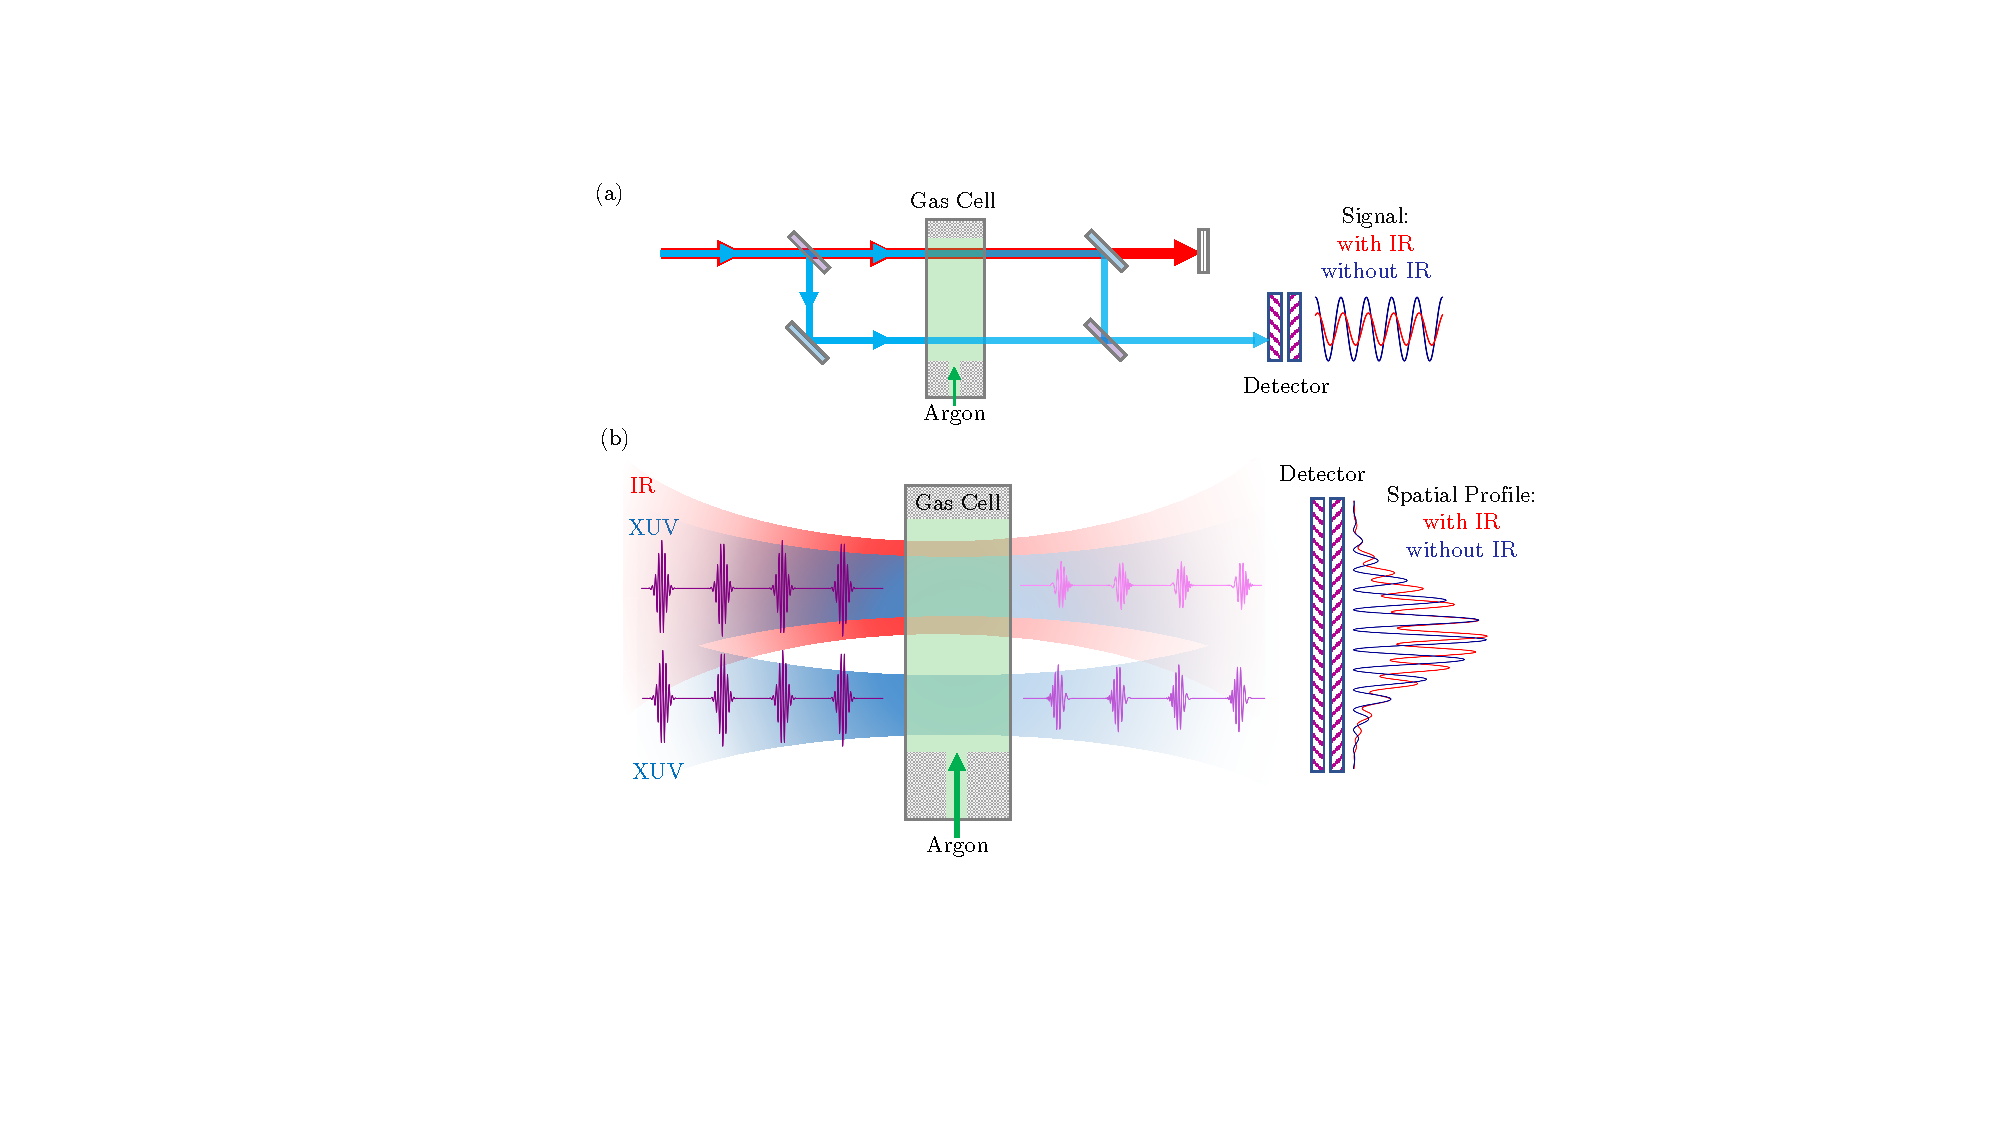
\includegraphics[width=1.0\textwidth]{figures/CATS/CATS_mach_zehnder.pdf}
	\caption[Schematic of Mach-Zehnder interferometer and spatial profile with and without an IR dressing field in one arm of the interferometer]{(a) Schematic of a Mach-Zehnder interferometer that is used to measure the phase shift induced by an IR dressing field introduced into one of the arms of the interferometer. (b) For the experiments described in this chapter, the two XUV sources generated by a SWPG will act as the two arms of a Mach-Zehnder interferometer, and the sample of interest will only be dressed in one the sources by an IR field.}
	\label{fig:CATS_mach-zehnder_interferometer}
\end{figure}

In the experiment presented in Chapter \ref{chap:refractive_index}, the complex refractive index that was measured corresponded to the ground state of a material.  However, this method can be generalized to measure more than just the static ground state, and it can be used to measure a dynamically induced change in refractive index via a dressing pulse.  The basic principle is shown schematically in figure \ref{fig:CATS_mach-zehnder_interferometer}, and it involves inducing a phase shift in only one arm of a Mach-Zehnder interferometer that is comprised of two nearly identical XUV beams going through the same medium. In a manner that is the same as what was presented in Chapter \ref{chap:refractive_index}, these two XUV beams will be generated by a SWPG.  The inherent interferometric stability of the SWPG due to its single-optic operation allows for measurements of phase shifts between the two beams that correspond to a delay of only a few attoseconds (see figure \ref{fig:interferogram_ge} for an example) that arise due to the change in the real refractive index induced by the dressing pulse.  The relationship between the change in the real refractive index, $\Delta n$, and the phase shift between the two beams, $\Delta\phi$, is given by
\begin{equation}
	\label{eqn:phase_shift_dn}
	\Delta \phi = \frac{2\pi L \Delta n}{\lambda}
\end{equation}
for a medium of length $L$.  This phase shift between the two beams is directly measured as a fringe shift in the spatial profile of interference pattern in the far-field, as was shown previously. This combined with a spectrometer allows for the measurement of the induced phase shift as a function of photon energy, and consequently, the real part of the refractive index can be measured as a function of photon energy.  

Additionally, the change in the imaginary part of the refractive index induced by the dressing pulse will lead to a change in absorption between the two beams, and this will lead to a change in fringe contrast in the far-field interference pattern.  The relationship between the change in contrast and the change in the imaginary refractive index, $\Delta \beta$,  is given by
\begin{equation}
	\label{eqn:beta_fringe_contrast_chap_cats}
	\Delta\beta = -\frac{c}{\omega L} \ln\Bigg[\frac{V_0}{V}\Bigg(1-\sqrt{1-\bigg(\frac{V}{V_0}\bigg)^2}\Bigg)\Bigg]
\end{equation}
where $V_0$ is the fringe contrast without the dressing pulse present and $V$ is the contrast with the dressing pulse present.  This change in imaginary part of the refractive index is related to the change in absorption, $\dod$, by the relationship
\begin{equation}
	\label{eqn:dod_to_beta}
	\dod(\omega) = \frac{2 \omega L}{c \ln 10}\Delta \beta(\omega),
\end{equation}
when the Beer-Lambert Law is assumed to hold true. 

Therefore, just as in the experiment performed in Chapter \ref{chap:refractive_index}, it is possible to directly measure the complex refractive index using a SWPG to generate an inline interferometer between two nearly identical XUV beams.  The primary difference is that now we are measuring only a change in the complex refractive index induced by a dressing pulse, as opposed to the total complex refractive index which would include the ground state.  This is due to the fact that this measurement is inherently differential in nature.  To measure the total complex refractive index, then one would have to limit the medium that is being dressed to only one of the two sources.  This is technically challenging for a gas sample, so only the change in complex refractive index is measured in this chapter.


\subsection{Indirect calculation: Kramers-Kronig Relations}

Beyond a direct measurement of both parts of the complex refractive index, there is another method that can be applied when only one of the two parts of the refractive index is measured, as is the case for a normal ATS experiment.  Namely, the Kramers-Kronig (KK) relations can be used to calculate one part from the other \cite{kronigTheoryDispersionXRays1926, kramersDiffusionLumierePar1927}.  These KK relations are Hilbert transforms that link the real and imaginary part of a complex function when some assumptions are met \cite{lucariniKramersKronigRelationsOptical2005}.  However, as will be examined later, their usefulness is limited in certain cases because they are not always directly applicable.


One of the powerful features of the KK relations is that they are fundamentally rooted in the assumption that causality holds true.  This can be seen in one of the two main methods of derivation \cite{hutchingsKramersKronigRelationsNonlinear1992, jacksonClassicalElectrodynamics1999, arfkenMathematicalMethodsPhysicists2013}, and will be briefly shown herein.   To begin, consider a dielectric medium under the influence of an electric field $\mathcal{E}(t)$.  The polarization $P(t)$ is then given by
\begin{equation}
	P(t)=\int_{-\infty}^{\infty}G(t')\mathcal{E}(t-t') \diff t'
\end{equation} 
where $G(t')$ is the Green's function that characterizes the response of the system to a $\delta$-function input.  In the frequency domain this equation is given by
\begin{equation}
	\tilde{P}(\omega)=\chi(\omega)\tilde{\mathcal{E}}(\omega),
\end{equation}
where the susceptibility is defined in terms of the response function as
\begin{equation}
	\chi(\omega)=\int_{-\infty}^{\infty}G(t')e^{i\omega t'}\diff t'.
\end{equation}
Now, invoking causality entails that the system cannot respond before the impulse.  If the impulse occurs at $t=0$, then the response must be zero for $t<0$.  Therefore, the Green's function is written as
\begin{equation}
	G(t)=G(t)\Theta(t)
\end{equation}
where $\Theta(t)$ is the Heaviside step function.  Fourier transforming this relationship yields
\begin{equation}
	\begin{aligned}
		\chi(\omega) &= \chi(\omega) \circledast \bigg(\frac{\delta(\omega)}{2} + \frac{i}{2\pi\omega}\bigg)\\
		& = \frac{\chi(\omega)}{2} + \frac{i}{2\pi} \mathrm{PV} \int_{-\infty}^{\infty}\frac{\chi(\omega')}{\omega - \omega'}\diff\omega'\\
		& = \frac{1}{i\pi} \mathrm{PV} \int_{-\infty}^{\infty}\frac{\chi(\omega')}{\omega' - \omega} \diff \omega'
	\end{aligned}
\end{equation}
where $\circledast$ represents convolution and  $\mathrm{PV}$ represents the Cauchy principal value.  Taking the real and imaginary parts of this equation yield the KK relations for the optical susceptibility, however they can be cast in terms of the refractive index by considering difference in output electric field betwen the two cases where the medium is present and the medium is absent.  The result of this is the KK relation linking the real and imaginary part of the refractive index, and this is given by
\begin{equation}
	\label{eqn:KK_n_beta}
	\tilde{n}(\omega) - 1 = \frac{2\omega}{\pi}\mathrm{PV}\int_{0}^{\infty} \frac{\tilde{\beta}(\omega')}{\omega'^2 - \omega^2} \diff \omega'.
\end{equation}
Using this relationship means that only one part of the refractive index needs to be measured to fully characterize both the real and imaginary parts of the refractive index.  This is a powerful tool because generally the imaginary part of the refractive index in much easier to experimentally measure.

However, there were some assumptions that were made in the derivation of the KK relation in equation \ref{eqn:KK_n_beta} that are important to scrutinize because they are not generally true.  The first assumption that was made was using the linear susceptibility $\chi(\omega)$.  By doing so we derived the linear KK relations, and these do not hold true when considering higher order nonlinear optical processes \cite{lucariniKramersKronigRelationsOptical2005, hutchingsKramersKronigRelationsNonlinear1992}.  For a higher order process, it is possible to derive KK relations that link the real and imaginary part, and these relations generally take the form given by
\begin{equation}
	\label{eqn:dn_db_KK}
	\Delta\tilde{n}(\omega, \zeta) = \frac{2\omega}{\pi} \mathrm{PV}\int_{0}^{\infty} \frac{\Delta\tilde{\beta}(\omega',\zeta)}{\omega'^2 - \omega^2} 
\end{equation}  
where $\Delta\tilde{n}(\omega, \zeta)$ and $\Delta\tilde{\beta}(\omega,\zeta)$ are the change in the real and imaginary refractive index due to a perturbation $\zeta$ \cite{hutchingsKramersKronigRelationsNonlinear1992, lucariniKramersKronigRelationsOptical2005}.  For an $n$-th order nonlinear process, these changes in the refractive index will generally be proportional to the real and imaginary parts of the $n$-th order nonlinear susceptibility $\chi^{(n)}$ \cite{boydNonlinearOptics2008, lucariniKramersKronigRelationsOptical2005, hutchingsKramersKronigRelationsNonlinear1992}.

Beyond the assumption of the linear susceptibility, another scenario in which the validity of the KK relations must be examined is the case of a pump-probe experiment \cite{tokunagaFemtosecondTimeresolvedDispersion1993, tokunagaFemtosecondContinuumInterferometer1996, lucariniKramersKronigRelationsOptical2005}.  Consider the change in polarization due to the pump pulse given by
\begin{equation}
	\Delta P(t) = \chi(t)\circledast \big( \mathcal{E}(t) \Delta N(t)\big) = \int_{0}^{\infty}\chi(t')\mathcal(t-t')\Delta N(t-t')
\end{equation}
where $\Delta N (t)$ represents the change in the medium due to the pump pulse.
\section{Complex Attosecond Transient-absorption Spectroscopy of Fano resonances}
\label{sec:CATS_ar}

\subsection{Experimental setup}
\label{sec:CATS_ar_exp_setup}

\begin{figure}
	\centering
	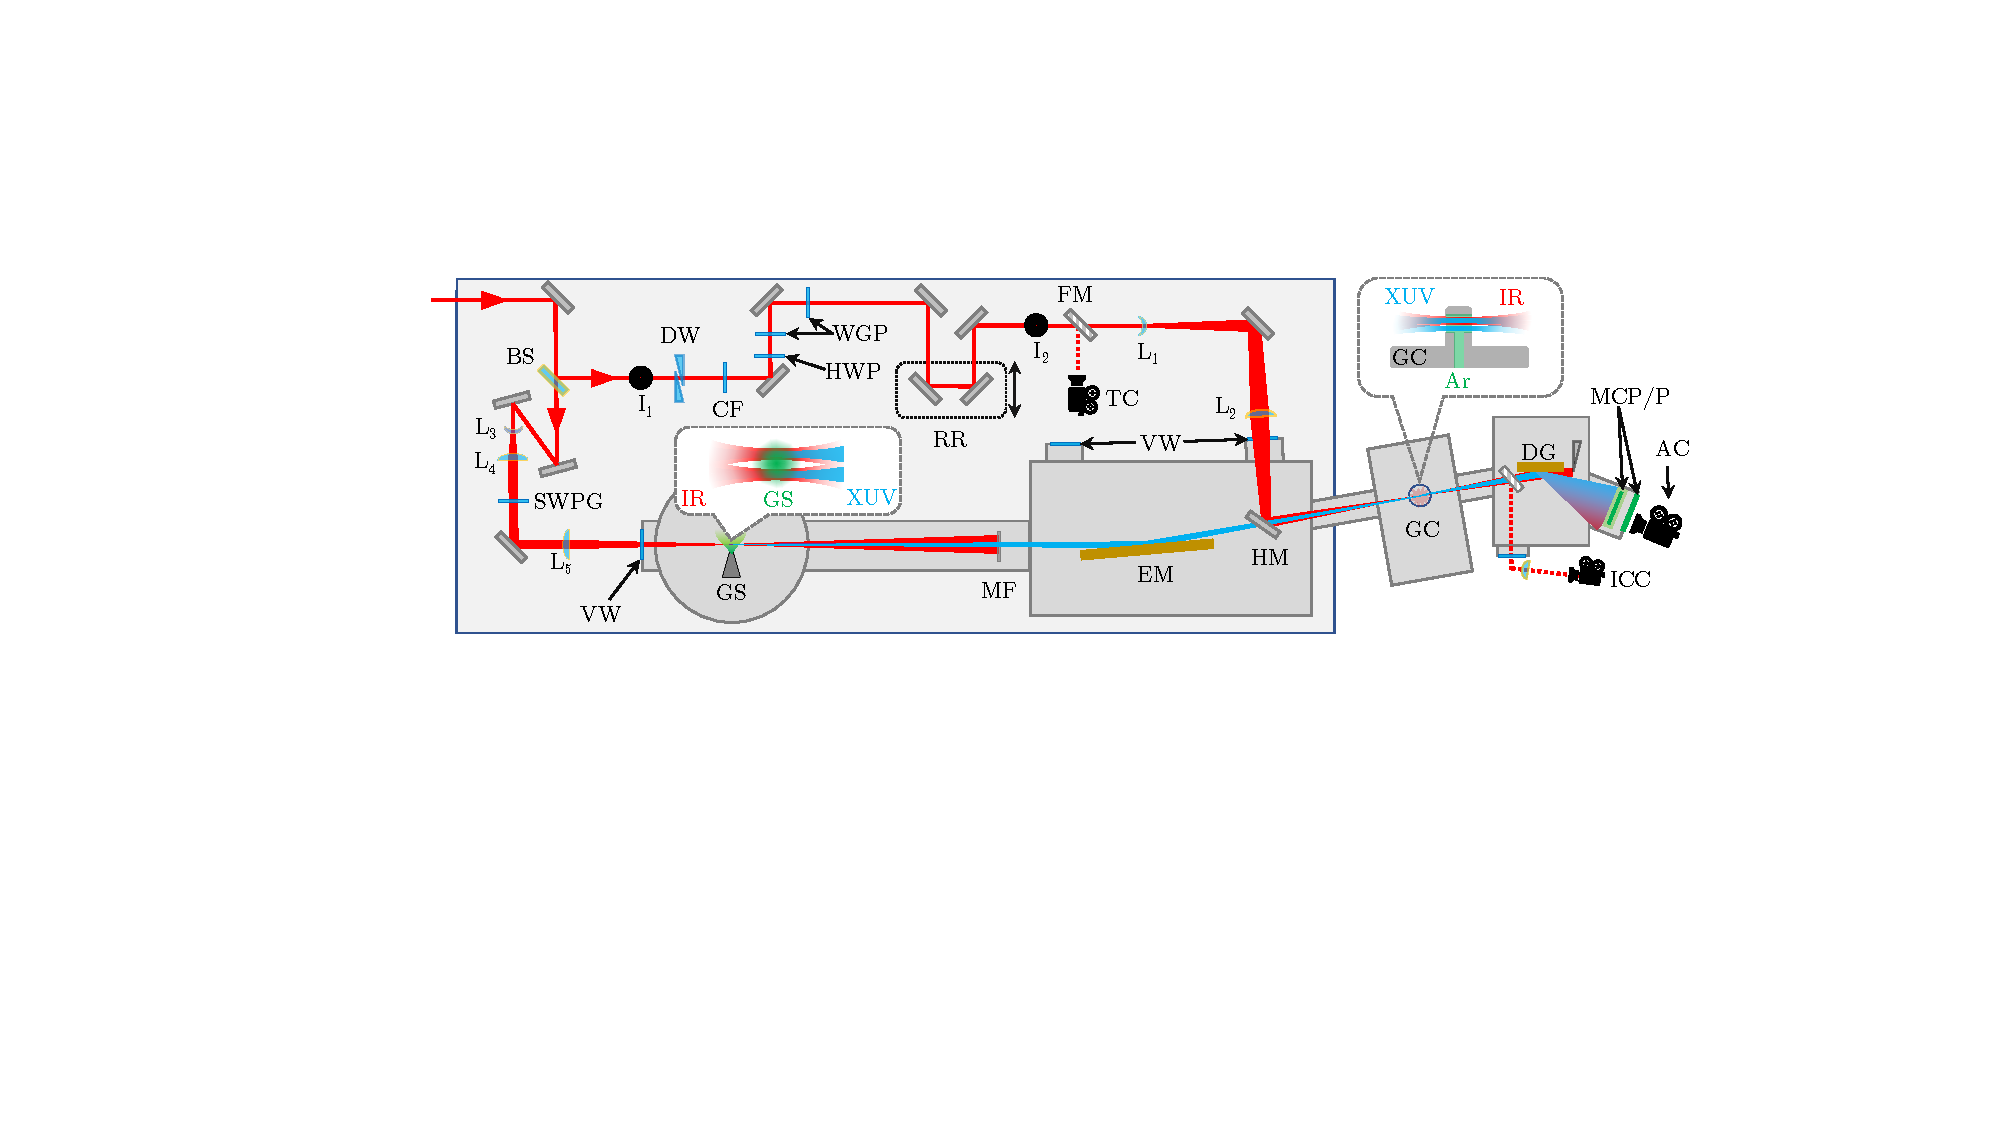
\includegraphics[width=1.0\textwidth]{figures/CATS/beamline_schematic_CATS.pdf}
	\caption[TABLe experimental setup for ATS experiments]{Schematic of the optical setup for the experiments described in this chapter.  \textbf{BS}: Beamsplitter (Thorlabs BSF20-C), \textbf{I$_{1,2}$}: Irises used for alignment. \textbf{DW}: Delay wedges for fine delay control. \textbf{CF}: Color filter (Thorlabs FELH1000). \textbf{HWP}: Half-wave plate. \textbf{WGP}: Wire grid polarizer. \textbf{RR}: Retro reflector for coarse delay adjustment.  \textbf{FM}: Flip mirror. \textbf{TC}: Thermal camera used for alignment.  \textbf{L$_1$}: $f=-300$ mm lens (Thorlabs LF1015-C). \textbf{L$_2$}: $f=500$ mm lens (Thorlabs LA1380-C). \textbf{VW}: Vacuum window, 3 mm CaF$_2$, \textbf{HM}: Hole mirror with 10 mm hole.  \textbf{L$_3$}: $f=-400$ mm lens.  \textbf{L$_4$}: $f=500$ mm lens. \textbf{L$_5$}: $f=400$ mm lens.  \textbf{BBO}: Second-harmonic generation crystal.  \textbf{Cal}: Calcite. \textbf{GS}: Gas source for HHG. \textbf{MF}: Aluminum filter. \textbf{EM}: Ellipsoidal mirror. \textbf{GC}: Gas cell. \textbf{RM}: Removable mirror for \textit{in-situ} diagnotics.    \textbf{ICC}: camera for \textit{in-situ} diagnotics. \textbf{DG}: VLS diffraction grating. \textbf{BB}: Baffles to block zero order diffraction.  \textbf{MCP/P}: Microchannel plate and phosphor.  \textbf{AC}: Andor Neo 5.5 CMOS camera.}
	\label{fig:CATS_setup}
\end{figure}



\subsection{Results}
\label{sec:CATS_ar_results}


\section{Conclusion}
\label{sec:CATS_conclusion}